\subsection{Approfondimenti}
Andiamo ad approfondire le azioni che è possibile fare tramite il terminale.
\subsubsection{Abbreviazione dei nomi}
È possibile abbreviare il nome del task da eseguire stando però attenti ad identificarlo unicamente, per esempio se volessi eseguire il task \textbf{dependenceTwo} potrei farlo semplicemente con il comando:
\begin{verbatim}
    $ gradle depTw \end{verbatim}
considerando i task creati precedentemente notiamo che il task è univocamente identificato.

\subsubsection{Escludere i task}
È possibile escludere un task di una build, aggiungendo come argomento il task da escludere preceduto da -x:
\begin{verbatim}
    $ gradle <task_da_eseguire> -x <task_da_escludere> \end{verbatim}
questo viene usato al fine di eliminare un task inutile per lo scopo della build che abbiamo intenzione di eseguire. Riprendendo l'output di \begin{verbatim}   $ gradle mainTask \end{verbatim} notiamo che vengono eseguiti tutti i tasks definiti nella build.gradle (a pagina \pageref{outMainTask}), se volessimo escludere dependenceOne dalla build allora dovremo eseguire:
\begin{verbatim}
    $ gradle mainTask -x dependenceOne \end{verbatim}
Otteniamo in questo modo in output:
\begin{verbatim}
> Task :dependenceTwo 
First Two
Last Two

> Task :mainTask 
First MainTask
Last MainTask


BUILD SUCCESSFUL in 0s
2 actionable tasks: 2 executed
\end{verbatim}
Possiamo notare che non verrà eseguito nemmeno il task dependenceZero perchè è una dipendenza del task dependenceOne.

\subsubsection{Selezionare la build da eseguire}
Consideriamo che esista in una subdirectory chiamata subdir una build chiamata subbild.gradle, partendo dalla directory source è possibile eseguire questa build eseguendo il comando:
\begin{verbatim}
    $ gradle -b subdir/subbuild.gradle <task_da_eseguire> \end{verbatim}
Questa particolare funzione serve soprattutto ai progetti multi-builds, in cui è necessario avere a disposizione più di una build di riferimento.

\subsubsection{Forzare l'esecuzione di un task} 
A causa della Gradle cache è possibile che un task o più di uno non vengano eseguiti perchè marcati come UP-TO-DATE (anche se dalla versione Gradle 4.0 non viene più mostrato in output), in questo caso è possibile forzarne l'esecuzione con:
\begin{verbatim}
    $ gradle --rerun-tasks <tasks_da_eseguire> \end{verbatim}
    
\subsubsection{Continuare la build quando si verifica un errore}
Se durante una build un task fallisce, Gradle di default interromperà l'esecuzione e farà fallire anche la build. Questo permette alla build di completare velocemente, ma il fallimento anticipato della build potrebbe nascondere altri problemi che possono presentarsi in altri tasks. A volte è quindi necessario imporre ad una build di gradle di continuare nonostante il fallimento di uno o più tasks, questo è possibile usando l'opzione \texttt{--continue}:
\begin{verbatim}
    $ gradle <tasks_da_eseguire> --continue\end{verbatim}
In questo modo verranno eseguiti tutti i tasks e solo al completamento della build saranno resi noti gli errori.

\subsubsection{Ottenere informazioni generali} 
Per visualizzare una lista dei principali tasks eseguibili è possibile eseguire il task \begin{verbatim}    $ gradle tasks\end{verbatim} l'output di questa build sarà:
\begin{verbatim}
> Task :tasks 

------------------------------------------------------------
All tasks runnable from root project - Example of Task
------------------------------------------------------------

Build Setup tasks
-----------------
init - Initializes a new Gradle build.
wrapper - Generates Gradle wrapper files.

Help tasks
----------
buildEnvironment - Displays all buildscript dependencies declared in root project 'src'.
components - Displays the components produced by root project 'src'. [incubating]
dependencies - Displays all dependencies declared in root project 'src'.
dependencyInsight - Displays the insight into a specific dependency in root project 'src'.
dependentComponents - Displays the dependent components of components in root project 'src'. 
[incubating]
help - Displays a help message.
model - Displays the configuration model of root project 'src'. [incubating]
projects - Displays the sub-projects of root project 'src'.
properties - Displays the properties of root project 'src'.
tasks - Displays the tasks runnable from root project 'src'.

To see all tasks and more detail, run gradle tasks --all

To see more detail about a task, run gradle help --task <task>


BUILD SUCCESSFUL in 0s
1 actionable task: 1 executed
\end{verbatim}

come dice l'output, per visualizzare la lista di tutti i tasks eseguibili nel nostro project è necessario eseguire la build del task \begin{verbatim}$ gradle tasks --all \end{verbatim} noteremo che in questo caso verranno visualizzati anche i tasks che abbiamo precedentemente creato (dependenceZero, dependenceOne, dependenceTwo, mainTask con le relative descrizioni):
\begin{verbatim}
> Task :tasks 

------------------------------------------------------------
All tasks runnable from root project - Example of Task
------------------------------------------------------------

Build Setup tasks
-----------------
init - Initializes a new Gradle build.
wrapper - Generates Gradle wrapper files.

Help tasks
----------
buildEnvironment - Displays all buildscript dependencies declared in root project 'src'.
components - Displays the components produced by root project 'src'. [incubating]
dependencies - Displays all dependencies declared in root project 'src'.
dependencyInsight - Displays the insight into a specific dependency in root project 'src'.
dependentComponents - Displays the dependent components of components in root project 'src'. 
[incubating]
help - Displays a help message.
model - Displays the configuration model of root project 'src'. [incubating]
projects - Displays the sub-projects of root project 'src'.
properties - Displays the properties of root project 'src'.
tasks - Displays the tasks runnable from root project 'src'.

Other tasks
-----------
dependenceOne - Build Dependence One
dependenceTwo - Build Dependence Two
dependenceZero - Build Dependence Zero
mainTask - Build Main Task


BUILD SUCCESSFUL in 0s
1 actionable task: 1 executed
\end{verbatim}
Se invece vogliamo informazioni più specifiche riguardo un singolo task la build da fare è 
\begin{verbatim}
    $ gradle help --task <nome_del_task>\end{verbatim}
per esempio eseguiamo:
\begin{verbatim}
    $ gradle help --task mainTask\end{verbatim}
otterremo una descrizione specifica del task mainTask:
\begin{verbatim}
> Task :help 
Detailed task information for mainTask

Path
     :mainTask

Type
     Task (org.gradle.api.Task)

Description
     Build Main Task

Group
     -\end{verbatim}

\subsubsection{Build scan}
Una funzione molto interessante di Gradle è la possibilità di poter pubblicare la propria build, questo permette di avere un report completo e condivisibile. Per utilizzare questa funzionalità è necessario aggiungere alla build di un task l'opzione \texttt{--scan}:
\begin{verbatim}    $ gradle <task_da_eseguire> --scan \end{verbatim}
Al completamento della build del task verrà richiesto di accettare i termini di uso di questo servizio. Una volta accettati verrà fornito un link alla build pubblicata in cui sarà richiesta una mail di riferimento per confermare la pubblicazione della build. Prendendo come esempio eseguiamo il comando:
\begin{verbatim}
    $ gradle mainTask --scan\end{verbatim}
l'output risultante sarà:
\begin{verbatim}
> Task :dependenceZero 
First Zero
Last Zero

> Task :dependenceOne 
First One
Last One

> Task :dependenceTwo 
First Two
Last Two

> Task :mainTask 
First MainTask
Last MainTask


BUILD SUCCESSFUL in 1s
4 actionable tasks: 4 executed

Publishing a build scan to scans.gradle.com requires accepting the Gradle Terms of Service 
defined at https://gradle.com/terms-of-service. Do you accept these terms? [yes, no] 
yes
Gradle Terms of Service accepted.

Publishing build scan...
https://scans.gradle.com/s/qcc4vkuegibig
\end{verbatim}
cliccando sul sito e seguendo le indicazioni, il risultato finale sarà:
\begin{figure}[H]
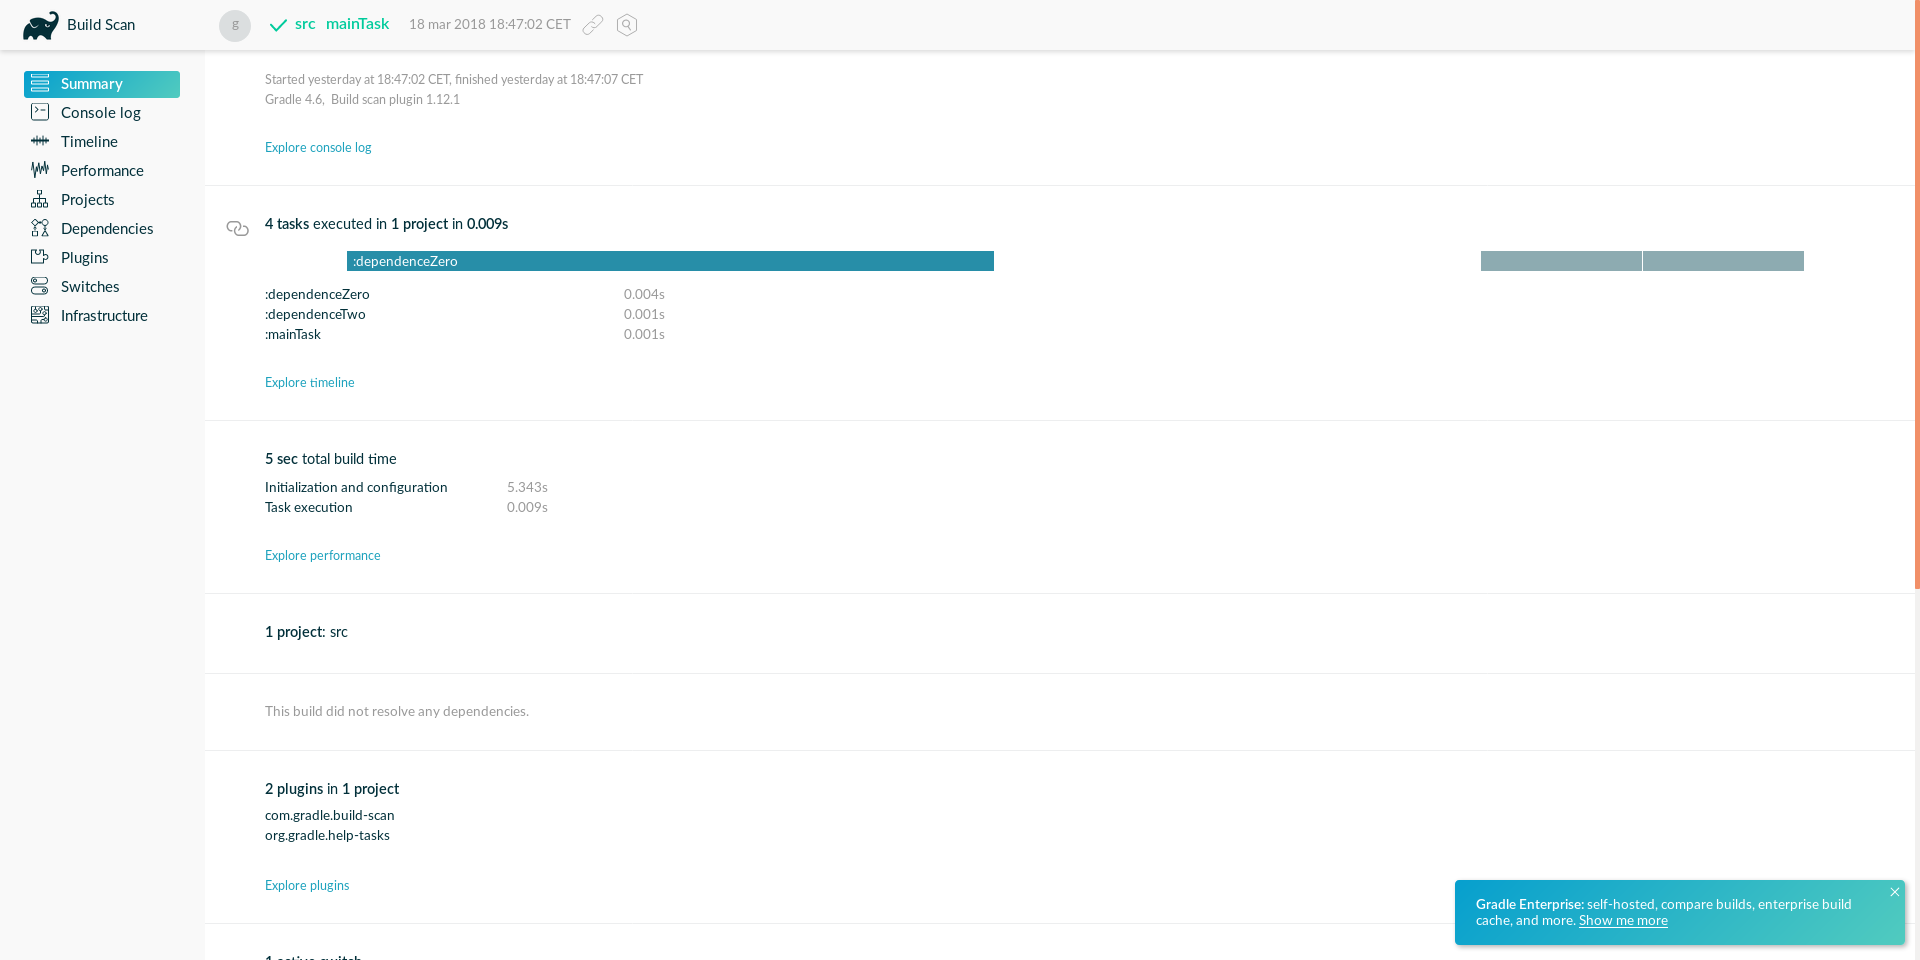
\includegraphics[scale=0.25]{1Task/insights/gradleScan.png}
\end{figure}